% Fuente autocontenida. Compilar dos veces con pdfLaTeX.
% Las tablas y graficas contienen resultados calculados por experimentos_rk4.py.
\documentclass[11pt,a4paper]{article}
\usepackage[utf8]{inputenc}
\usepackage[T1]{fontenc}
\usepackage[provide=*,spanish]{babel}
\usepackage{lmodern,microtype}
\usepackage[margin=2.25cm,headheight=15pt]{geometry}
\usepackage{amsmath,amssymb,amsthm,mathtools,bm}
\usepackage{booktabs,tabularx,longtable,array}
\usepackage{enumitem,xcolor,fancyhdr,titlesec}
\usepackage[most]{tcolorbox}
\usepackage{tikz,pgfplots,listings}
\pgfplotsset{compat=1.18}
\usepackage[colorlinks=true,linkcolor=navy,urlcolor=teal,citecolor=teal]{hyperref}
\definecolor{navy}{HTML}{16324F}
\definecolor{teal}{HTML}{007F82}
\definecolor{pale}{HTML}{EDF5F5}
\definecolor{graytext}{HTML}{526273}
\hypersetup{pdftitle={RK4 vectorial: condiciones iniciales aleatorias y paso adaptativo},pdfauthor={José Carlos Torres Donaire}}
\titleformat{\section}{\Large\bfseries\color{navy}}{\thesection}{0.7em}{}
\titleformat{\subsection}{\large\bfseries\color{navy}}{\thesubsection}{0.6em}{}
\pagestyle{fancy}\fancyhf{}
\fancyhead[L]{\small\color{graytext}RK4 vectorial y propagación de incertidumbre}
\fancyhead[R]{\small\color{graytext}Informe técnico}
\fancyfoot[C]{\small\thepage}
\renewcommand{\headrulewidth}{0.3pt}
\setlength{\parindent}{0pt}\setlength{\parskip}{6pt}
\setlist{itemsep=3pt,topsep=4pt}
\newtheorem{theorem}{Teorema}[section]
\newtheorem{proposition}[theorem]{Proposición}
\newtheorem{lemma}[theorem]{Lema}
\theoremstyle{definition}\newtheorem{definition}[theorem]{Definición}
\theoremstyle{remark}\newtheorem{remark}[theorem]{Observación}
\newcommand{\R}{\mathbb R}\newcommand{\E}{\mathbb E}
\newcommand{\Prob}{\mathbb P}\newcommand{\norm}[1]{\left\lVert#1\right\rVert}
\newcommand{\Cov}{\operatorname{Cov}}\newcommand{\Law}{\mathcal L}
\newcommand{\diag}{\operatorname{diag}}\newcommand{\atol}{\mathrm{atol}}
\newcommand{\rtol}{\mathrm{rtol}}
\newtcolorbox{keybox}[1]{colback=pale,colframe=teal,boxrule=0.5pt,arc=1mm,title=#1,fonttitle=\bfseries,breakable}
\lstset{basicstyle=\ttfamily\small,breaklines=true,frame=single,rulecolor=\color{teal},backgroundcolor=\color{pale},columns=fullflexible,keepspaces=true,showstringspaces=false}
\begin{document}
\begin{titlepage}
\vspace*{1.2cm}
{\color{teal}\large ANÁLISIS NUMÉRICO Y ECUACIONES DIFERENCIALES}\par
\vspace{1.1cm}
{\color{navy}\fontsize{30}{35}\selectfont\bfseries Runge--Kutta de\par cuarto orden\par para sistemas vectoriales}\par
\vspace{0.65cm}
{\Large Condiciones iniciales aleatorias,\par paso adaptativo y estado del arte}\par
\vspace{1cm}
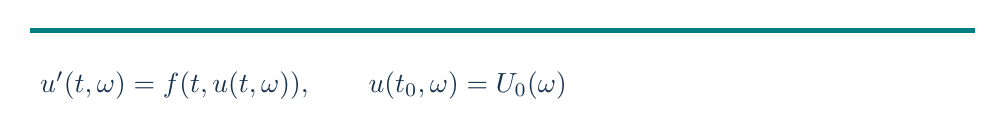
\begin{tikzpicture}
\draw[teal,line width=2pt] (0,0)--(12,0);
\node[anchor=west,text=navy] at (0,-0.7) {$u'(t,\omega)=f(t,u(t,\omega)),\qquad u(t_0,\omega)=U_0(\omega)$};
\end{tikzpicture}\par
\vspace{1.3cm}
{\large José Carlos Torres Donaire}\par
Universidad Nacional Autónoma de Honduras\par
Ingeniería en Sistemas\par
\vfill
\begin{keybox}{Alcance del trabajo}
Formulación en dimensión arbitraria, verificación de las condiciones de orden,
demostraciones de convergencia, propagación probabilística y diseño de un
integrador adaptativo. Incluye una revisión crítica de literatura y experimentos
ejecutados con código reproducible. Los ejemplos verifican la teoría y no
restringen la clase de problemas estudiada.
\end{keybox}
\vspace{0.5cm}
{\color{graytext}13 de octubre de 2026\par Informe y material de apoyo para exposición}
\end{titlepage}
\section*{Resumen}
\addcontentsline{toc}{section}{Resumen}
Este trabajo estudia el método clásico de Runge--Kutta de cuarto orden (RK4)
para problemas de valor inicial en $\R^d$, con especial atención a dos
extensiones: la incertidumbre en el dato inicial y la selección automática del
paso temporal. El análisis parte de una formulación vectorial general y
distingue la aleatoriedad del modelo, la aleatoriedad de las entradas y la
incertidumbre introducida por la discretización. Se verifican las ocho
condiciones algebraicas de orden hasta cuatro, se establece una cota de error
global en mallas no uniformes y se extiende esa cota a normas de Bochner y a
distancias de Wasserstein bajo hipótesis explícitas. Para la adaptatividad se
deriva el estimador por duplicación de paso, incluido el factor $15$ y el
exponente $1/5$ del controlador. Se examinan los límites del control local, la
rigidez y la comparación con pares embebidos. La revisión bibliográfica
relaciona estas ideas con integradores probabilísticos, controladores PI/PID
y conservación de invariantes, evitando identificar estas líneas con RK4
clásico. Se complementa el desarrollo con experimentos vectoriales, un
ensamble de condiciones iniciales gaussianas y una verificación estocástica
de Euler--Maruyama con trayectorias brownianas acopladas.

\textbf{Palabras clave:} RK4, EDO vectoriales, condiciones iniciales aleatorias,
paso adaptativo, convergencia, Monte Carlo, incertidumbre numérica.

\begin{keybox}{Resultado principal}
La misma fórmula RK4 se aplica a cada realización del dato inicial. Bajo
regularidad y control uniforme de los defectos locales, su error global es
$O(h_*^4)$, donde $h_*$ es el mayor paso aceptado. La aleatoriedad inicial
no exige agregar incrementos brownianos. Un controlador adaptativo regula
un estimador local y no constituye, por sí solo, una certificación global.
\end{keybox}
\clearpage
\setcounter{tocdepth}{1}
\tableofcontents
\clearpage
\section{Interpretación y cumplimiento de la asignación}
El documento de asignación solicita RK4 para una EDO vectorial, una extensión
con condiciones iniciales aleatorias y otra con paso $h$ adaptativo. También
pide un estado del arte en arXiv y exploración de artículos relacionados,
con la advertencia de no limitarse a casos especiales. Finalmente menciona
Euler vectorial y Euler--Maruyama. El presente informe desarrolla estos
componentes con una notación consistente y acompaña el informe con una
presentación en LaTeX.

\begin{center}\small
\begin{tabularx}{\linewidth}{@{}p{4.3cm}X@{}}\toprule
Requisito & Desarrollo en este trabajo\\\midrule
EDO vectorial general & $f:[t_0,T]\times\R^d\to\R^d$, sin fijar dimensión ni una aplicación concreta.\\
RK4 y computación & Tabla de Butcher, condiciones de orden, convergencia y algoritmos.\\
Condición inicial aleatoria & Flujo aleatorio, ley transportada, momentos y estimación Monte Carlo.\\
Paso adaptativo & Duplicación de paso, norma escalada, aceptación/rechazo y control del paso.\\
Estado del arte & Fuentes primarias verificables, matriz crítica y conexiones temáticas.\\
Euler y Euler--Maruyama & Comparación determinista y delimitación de la extensión estocástica.\\
Entrega & Informe y presentación autocontenidos en \texttt{.tex} y \texttt{.pdf}; código y resultados reproducibles.\\\bottomrule
\end{tabularx}\end{center}

\subsection{Corrección de la notación de partida}
Para una EDO, el argumento del campo vectorial es el estado y se escribe
$u'=f(t,u)$. La notación $u(t,x)$ puede representar una familia parametrizada
por un dato inicial $x$, pero no implica derivadas espaciales. Si $x$ fuese
una coordenada espacial y el modelo incluyera derivadas respecto de $x$, se
trataría de una EDP o de su discretización espacial. Aquí $u(t;z)$ representa
la solución iniciada en $z\in\R^d$, mientras $u(t,\omega)$ representa una
realización aleatoria.

\subsection{Preguntas que organiza el análisis}
\begin{enumerate}
\item ¿Qué hipótesis permiten garantizar cuarto orden para un sistema acoplado?
\item ¿Qué conserva RK4 cuando el dato inicial es una variable aleatoria?
\item ¿Cómo estimar el error sin disponer de la solución exacta y cómo elegir $h$?
\item ¿Cómo separar el error temporal del error estadístico de Monte Carlo?
\item ¿Cuándo corresponde usar Euler--Maruyama y cuándo basta RK4 trayectoria por trayectoria?
\end{enumerate}
El objetivo es dar respuestas matemáticas generales. Los ensayos posteriores
ilustran su verificación; no se presentan como pruebas universales ni como
una evaluación exhaustiva de todos los integradores disponibles.

\clearpage
\section{Problema general, flujo y regularidad}
\subsection{Sistema determinista}
Sea $I=[t_0,T]$, $d\geq1$ y considérese
\begin{equation}\label{eq:ivp}
 u'(t)=f(t,u(t)),\qquad u(t_0)=z\in\R^d.
\end{equation}
Un sistema acoplado tiene componentes $f_i(t,u_1,\ldots,u_d)$. Todas las
etapas de un método explícito deben calcularse usando un mismo vector de
etapa, no actualizando componentes secuencialmente con valores mezclados.

Si $f$ es continua en $t$ y localmente Lipschitz respecto de $u$, existe una
solución local única. Para trabajar en todo $I$, se requiere además que la
solución no explote antes de $T$. Una condición suficiente es Lipschitz
global junto con $\sup_{t\in I}\norm{f(t,0)}<\infty$. Para las estimaciones de
cuarto orden se supondrá regularidad $C^5$ y cotas sobre las derivadas en un
entorno de las trayectorias y de las etapas numéricas consideradas. No basta
la existencia de una solución para afirmar cuarto orden.

\begin{definition}[Flujo]
La aplicación $\varphi_{t,s}(z)$ devuelve el valor en $t$ de la solución que
toma el valor $z$ en $s$. Su propiedad de composición es
$\varphi_{t,s}\circ\varphi_{s,r}=\varphi_{t,r}$ en los dominios donde las
soluciones existen.
\end{definition}
Si $f$ tiene constante Lipschitz $L$ en una región común, Grönwall da
\begin{equation}\label{eq:flow}
 \norm{\varphi_{t,t_0}(z)-\varphi_{t,t_0}(w)}
 \leq e^{L(t-t_0)}\norm{z-w}.
\end{equation}
Esta desigualdad relaciona la sensibilidad al dato inicial con la
amplificación del error numérico. En horizontes largos puede ser muy
conservadora; no garantiza que un sistema caótico mantenga trayectorias
individuales cercanas indefinidamente.

\subsection{Autonomización y dimensión arbitraria}
Definiendo $v=(t,u)$, la EDO no autónoma se transforma en
\[
 v'=F(v),\qquad F(t,u)=(1,f(t,u)).
\]
Así, las condiciones de orden para sistemas autónomos se trasladan al caso
no autónomo si $c=A\mathbf1$. Las operaciones de RK4 siguen siendo sumas de
vectores y evaluaciones de $f$; no requieren diagonalización ni solución de
sistemas algebraicos. La teoría clásica proporciona el marco general de
estos métodos \cite{hairer}.

\subsection{Tres fuentes distintas de incertidumbre}
\begin{center}\small
\begin{tabularx}{\linewidth}{@{}p{3.4cm}XX@{}}\toprule
Fuente & Modelo & Tratamiento\\\midrule
Dato inicial & $U_0$ tiene una ley prescrita & Transportar esa ley por el flujo; RK4 por realización.\\
Discretización & Se desconoce el error del integrador & Refinamiento, estimadores, residuos o métodos probabilísticos.\\
Ruido dinámico & $\mathrm dX=a\,\mathrm dt+B\,\mathrm dW$ & Integración estocástica, por ejemplo Euler--Maruyama.\\\bottomrule
\end{tabularx}\end{center}
Estas fuentes pueden coexistir, pero tienen interpretaciones y algoritmos
diferentes. La covarianza de un filtro numérico probabilístico no se identifica
automáticamente con la covarianza física inducida por $U_0$.

\clearpage
\section{RK4 vectorial y verificación del orden}
\subsection{Fórmula de cuatro etapas}
Sea $h_n=t_{n+1}-t_n>0$. Con la convención de incrementos, cada $k_i$
incluye el factor $h_n$:
\begin{align}
k_1&=h_n f(t_n,u_n),\\
k_2&=h_n f(t_n+h_n/2,u_n+k_1/2),\\
k_3&=h_n f(t_n+h_n/2,u_n+k_2/2),\\
k_4&=h_n f(t_n+h_n,u_n+k_3),\\
u_{n+1}&=u_n+\frac16(k_1+2k_2+2k_3+k_4)
          =:\Psi_{h_n}(t_n,u_n).\label{eq:rk4}
\end{align}
Si se definen etapas como pendientes $K_i=f(\cdots)$, entonces debe aparecer
un factor $h_n$ fuera de la suma final. Mezclar ambas convenciones agrega o
elimina erróneamente un factor de paso.

\subsection{Tabla de Butcher}
\[
\begin{array}{c|rrrr}
0&0&0&0&0\\
\tfrac12&\tfrac12&0&0&0\\
\tfrac12&0&\tfrac12&0&0\\
1&0&0&1&0\\\hline
&\tfrac16&\tfrac13&\tfrac13&\tfrac16
\end{array}
\]
Escribamos $A=(a_{ij})$, $b=(1/6,1/3,1/3,1/6)^\top$,
$c=A\mathbf1=(0,1/2,1/2,1)^\top$ y $C=\diag(c)$.
Las potencias de $c$ en la tabla siguiente son componente a componente.

\begin{center}
\begin{tabular}{@{}clc@{}}\toprule
Orden & Condición & Valor de RK4\\\midrule
1 & $b^\top\mathbf1=1$ & $1$\\
2 & $b^\top c=1/2$ & $1/2$\\
3 & $b^\top c^2=1/3$ & $1/3$\\
3 & $b^\top Ac=1/6$ & $1/6$\\
4 & $b^\top c^3=1/4$ & $1/4$\\
4 & $b^\top CAc=1/8$ & $1/8$\\
4 & $b^\top Ac^2=1/12$ & $1/12$\\
4 & $b^\top A^2c=1/24$ & $1/24$\\\bottomrule
\end{tabular}
\end{center}
Por ejemplo, $Ac=(0,0,1/4,1/2)^\top$ y
$A^2c=(0,0,0,1/4)^\top$, de donde
$b^\top Ac=1/6$ y $b^\top A^2c=1/24$.
Los ocho valores se verificaron adicionalmente con aritmética racional exacta.

\subsection{Por qué la verificación es vectorial}
La expansión de Taylor del flujo autónomo contiene diferenciales elementales
asociadas a los árboles enraizados de órdenes uno a cuatro. Al desarrollar
las etapas de RK, sus coeficientes son precisamente las ocho combinaciones
anteriores. La igualdad de estos coeficientes hace coincidir el flujo y el
método hasta los términos de grado cuatro, independientemente de $d$.
La autonomización extiende la conclusión a $f(t,u)$. Verificar únicamente
la ecuación escalar lineal no comprobaría las condiciones correspondientes
a derivadas mixtas y a ramificaciones no lineales.

\clearpage
\section{Convergencia en mallas no uniformes y estabilidad}
\begin{theorem}[Error global de RK4]\label{thm:global}
Supóngase que las soluciones y etapas permanecen en una región donde el
defecto local satisface
\[
 \norm{\varphi_{t+h,t}(y)-\Psi_h(t,y)}\leq C_{\mathrm{loc}}h^5
\]
y donde $\norm{\Psi_h(t,y)-\Psi_h(t,z)}\leq(1+Kh)\norm{y-z}$
para $0<h\leq\bar h$, con constantes uniformes $K\geq0$ y
$C_{\mathrm{loc}}\geq0$. Sea
$h_* =\max_n h_n\leq\bar h$ y $e_n=\norm{u(t_n)-u_n}$. Entonces
\begin{equation}\label{eq:global}
 \max_{0\leq n\leq N}e_n
 \leq e^{K(T-t_0)}\bigl(e_0+C_{\mathrm{loc}}(T-t_0)h_*^4\bigr).
\end{equation}
En particular, con dato inicial exacto, el método tiene orden global cuatro.
\end{theorem}
\begin{proof}
La consistencia de cuarto orden deriva de las condiciones anteriores y de
la regularidad que permite acotar el resto de Taylor. Por suma y resta de
$\Psi_{h_n}(t_n,u(t_n))$,
\[
 e_{n+1}\leq(1+Kh_n)e_n+C_{\mathrm{loc}}h_n^5.
\]
Iterando esta recurrencia y usando $1+Kh_n\leq e^{Kh_n}$ se obtiene
\[
e_n\leq e^{K(t_n-t_0)}
\left(e_0+C_{\mathrm{loc}}\sum_{j<n}h_j^5\right).
\]
Finalmente $\sum_j h_j^5\leq h_*^4\sum_j h_j=h_*^4(T-t_0)$.
No se requiere uniformidad de la malla ni una cota inferior global para $h_n$.
\end{proof}
\begin{remark}
Si $f$ es $L$-Lipschitz, las etapas proporcionan la cota de propagación
$1+Lh+(Lh)^2/2+(Lh)^3/6+(Lh)^4/24$. En un intervalo acotado de pasos esta
expresión es menor o igual que $1+Kh$ para una constante $K$ fija. La cota
del teorema es condicional a que las etapas permanezcan en la región de
regularidad. No se extiende automáticamente a campos discontinuos.
\end{remark}

\subsection{Estabilidad absoluta y rigidez}
Para $u'=\lambda u$, $z=\lambda h$,
\[
R_{\mathrm{RK4}}(z)=1+z+\frac{z^2}{2}+\frac{z^3}{6}+\frac{z^4}{24},
\qquad R_{\mathrm E}(z)=1+z.
\]
El dominio de estabilidad absoluta es $\{z\in\mathbb C:|R(z)|\leq1\}$.
Sobre el eje real negativo, RK4 admite aproximadamente
$z\in[-2.785293,0]$ y Euler $z\in[-2,0]$. Para
$u'=Au$, la actualización es $u_{n+1}=R(hA)u_n$. Si $A$ es normal, el
análisis espectral caracteriza la norma euclídea inducida de este polinomio; en matrices no
normales puede existir crecimiento transitorio aun con espectro estable.

En problemas rígidos, la restricción de estabilidad puede exigir pasos
mucho menores que los requeridos por precisión. La adaptatividad no vuelve
A-estable a RK4. Métodos implícitos, como Radau o BDF, son alternativas que
deben evaluarse según el problema. Tampoco la mayor precisión asintótica
de RK4 garantiza superioridad frente a Euler para toda tolerancia, costo,
regularidad o propiedad cualitativa.

\clearpage
\section{Extensión I: condiciones iniciales aleatorias}
\subsection{Formulación trayectoria por trayectoria}
En un espacio de probabilidad $(\Omega,\mathcal F,\Prob)$, sea
$U_0:\Omega\to\R^d$ medible. Definimos
\begin{equation}\label{eq:random}
 u'(t,\omega)=f(t,u(t,\omega)),\qquad
 u(t_0,\omega)=U_0(\omega),\qquad
 u(t,\omega)=\varphi_{t,t_0}(U_0(\omega)).
\end{equation}
Si el flujo es continuo en el dato inicial, su composición con $U_0$ es
medible. Bajo las hipótesis de existencia anteriores, cada realización
resuelve una EDO determinista. Para RK4 basta tomar $U_0$ como vector inicial
y aplicar \eqref{eq:rk4} sin volver a muestrear ese dato durante la trayectoria.

La ley $\mu_t=\Law(u(t))$ es la medida transportada
\[
 \mu_t=(\varphi_{t,t_0})_\#\mu_0,
 \qquad \mu_t(B)=\mu_0(\varphi_{t,t_0}^{-1}(B)).
\]
Si existe una densidad suficientemente regular $\rho$, esta satisface en
sentido apropiado la ecuación de transporte
\[
 \partial_t\rho+\nabla_u\!\cdot(f(t,u)\rho)=0.
\]
No aparece un término de difusión a menos que se introduzca un mecanismo
de ruido dinámico en el modelo.

\subsection{Momentos y ausencia de cierre general}
Si la integrabilidad permite intercambiar derivada y esperanza,
\[
 m'(t)=\E[f(t,u(t))],\qquad m(t)=\E[u(t)].
\]
En general $\E[f(t,u)]\neq f(t,\E[u])$. Sea
$\Sigma(t)=\E[(u-m)(u-m)^\top]$. Como $\E[u-m]=0$,
\[
 \Sigma'=\E\!\left[f(t,u)(u-m)^\top+(u-m)f(t,u)^\top\right].
\]
Estas relaciones no forman un sistema cerrado para $(m,\Sigma)$ en un
campo no lineal arbitrario. Para $f(t,u)=A(t)u+b(t)$ sí se cierran:
\[
 m'=Am+b,\qquad\Sigma'=A\Sigma+\Sigma A^\top.
\]
El caso lineal resulta útil para verificar momentos, pero la metodología de
integración por realizaciones no requiere linealidad ni gaussianidad.

\subsection{Sensibilidad y aproximación local de covarianza}
Para $J(t,z)=D_z\varphi_{t,t_0}(z)$,
\[
 J'=D_uf(t,u(t;z))J,\qquad J(t_0,z)=I_d.
\]
Si $U_0$ está concentrado alrededor de $m_0$, la linealización sugiere
$\Sigma(t)\approx J(t,m_0)\Sigma_0J(t,m_0)^\top$.
Es una aproximación local, exacta en la situación afín, y puede resultar
inadecuada para distribuciones amplias o multimodales. Monte Carlo evita
este cierre a costa de un error de muestreo explícito.

\clearpage
\section{Convergencia probabilística y error estadístico}
\begin{theorem}[Extensión a $L^p$ y a la ley]\label{thm:lp}
Sea $1\leq p<\infty$. Supóngase que, para cada realización y para los nodos
de su malla, el error con dato inicial exacto satisface
\[
 \max_n\norm{u(t_n,\omega)-U_n(\omega)}
 \leq C(\omega)h_*(\omega)^4.
\]
Si $C\in L^p(\Omega)$ y $h_*(\omega)\leq\varepsilon$ casi seguramente,
entonces
\[
 \left\|\max_n\norm{u(t_n)-U_n}\right\|_{L^p}
 \leq\norm{C}_{L^p}\varepsilon^4.
\]
Si todos los caminos alcanzan un tiempo determinista $T$, sus leyes finales
satisfacen
\[
W_p(\Law(u(T)),\Law(U_T))\leq\norm{C}_{L^p}\varepsilon^4,
\]
siempre que existan los momentos de orden $p$ correspondientes.
\end{theorem}
\begin{proof}
Se eleva la cota trayectoria por trayectoria a la potencia $p$ y se integra.
Para Wasserstein se utiliza el acoplamiento que emplea el mismo $U_0$ en
la trayectoria exacta y la aproximada: por definición del ínfimo sobre
acoplamientos, $W_p\leq(\E\norm{u(T)-U_T}^p)^{1/p}$.
\end{proof}
Si $U_0$ tiene soporte compacto y las cotas del teorema
\ref{thm:global} son uniformes sobre la región alcanzable, $C$ puede ser
determinista. Para leyes gaussianas, el soporte no es compacto: se necesitan
cotas de crecimiento del error y suficientes momentos, o un argumento de
truncamiento con control explícito de las colas. La convergencia casi segura
por sí sola no implica convergencia en $L^p$.

\subsection{Monte Carlo y descomposición del error}
Sean $Z_1,\ldots,Z_M$ independientes con ley $\mu_0$ y sea $q:\R^d\to\R$
una cantidad de interés. Para un algoritmo determinista por realización,
\[
 Q_M^h=\frac1M\sum_{j=1}^M q(U_T^{(j)}),
 \qquad Q=\E[q(u(T))].
\]
Si $q$ es Lipschitz, el sesgo temporal satisface
$|\E[q(U_T)]-Q|\leq\operatorname{Lip}(q)\norm{u(T)-U_T}_{L^1}$.
Si además $q(U_T)\in L^2(\Omega)$, la identidad de error cuadrático medio es
\begin{equation}\label{eq:mse}
 \E[(Q_M^h-Q)^2]
 =\frac{\operatorname{Var}(q(U_T))}{M}
  +\left(\E[q(U_T)]-Q\right)^2.
\end{equation}
Por tanto, con la cota temporal anterior y una varianza acotada uniformemente
al refinar, el error RMS es $O(M^{-1/2}+h_*^4)$. Para observables indicadores, cuantiles o funciones
discontinuas, la cota Lipschitz no aplica directamente. Un intervalo normal
basado en $s/\sqrt M$ cuantifica muestreo asintótico, pero no incluye
automáticamente sesgo temporal ni error de modelo.

\subsection{Elección conjunta de $M$ y resolución temporal}
Un cálculo eficiente equilibra ambas contribuciones. Reducir $h$ cuando
$M^{-1/2}$ domina produce poca mejora estadística. Si el costo por trayectoria
es proporcional a $h^{-1}$, alcanzar un error objetivo $\eta$ con
$h=O(\eta^{1/4})$ y $M=O(\eta^{-2})$ sugiere un costo
$O(\eta^{-9/4})$ en este modelo simplificado. Esta cuenta ignora costos de
rechazo, rigidez, evaluación del campo y posibles métodos de reducción de
varianza; sirve como criterio de diseño, no como ley universal de complejidad.

\clearpage
\section{Extensión II: paso adaptativo para RK4}
\subsection{Derivación del estimador por duplicación}
Desde el mismo $(t,y)$ se calculan
\[
 y_c=\Psi_h(t,y),\qquad
 y_f=\Psi_{h/2}\bigl(t+h/2,\Psi_{h/2}(t,y)\bigr).
\]
Sea $y_*=\varphi_{t+h,t}(y)$. En el régimen asintótico suave,
\[
 y_c=y_*+C h^5+O(h^6),\qquad
 y_f=y_*+\frac{C}{16}h^5+O(h^6).
\]
La segunda expresión acumula dos defectos de tamaño $(h/2)^5$ y su
propagación cambia únicamente términos de orden superior. Por resta,
\begin{equation}\label{eq:estimator}
 \widehat e_f=\frac{y_f-y_c}{15}=y_*-y_f+O(h^6).
\end{equation}
El factor es $2^4-1=15$. Si se acepta $y_f$, se conserva un algoritmo
global de orden cuatro. La corrección de Richardson
$y_R=y_f+(y_f-y_c)/15$ cancela el término principal y puede elevar el orden
bajo regularidad suficiente, pero constituye otro algoritmo. Aquí se acepta
$y_f$ sin extrapolación para estudiar RK4 de manera consistente.

\subsection{Escalas y aceptación}
Para componentes con magnitudes diferentes, se utilizan
\[
 s_i=\atol_i+\rtol\max(|y_i|,|(y_f)_i|),\qquad
 r=\max_{1\leq i\leq d}\frac{|(\widehat e_f)_i|}{s_i}.
\]
Se acepta el paso si $r\leq1$; en caso contrario se conserva $(t,y)$ y se
repite el intento con menor $h$. Es necesario $s_i>0$: una tolerancia relativa
sin tolerancia absoluta falla cerca de componentes nulas. La norma infinito
controla todas las componentes escaladas. La norma RMS es otra elección
habitual, pero puede ocultar un error localizado cuando $d$ es grande.

Como $\widehat e_f=O(h^5)$, el controlador integral elemental es
\begin{equation}\label{eq:controller}
h_{\mathrm{nuevo}}=h\,\min\!\left(f_{\max},\max\!\left(f_{\min},
 \gamma r^{-1/5}\right)\right),\qquad 0<\gamma<1.
\end{equation}
En el código se usa $\gamma=0.9$, $f_{\min}=0.2$, $f_{\max}=5$.
Para $r=0$ se toma el máximo crecimiento permitido; tras un rechazo no se
permite aumentar el paso. El método realiza doce evaluaciones de $f$ por
intento en su implementación directa. Reutilizar la primera evaluación
compartida reduce ese costo a once; el código entregado no aplica esa
optimización y reporta el costo real.

\subsection{Lo que regula una tolerancia}
Aceptar $r\leq1$ no demuestra que el error global sea menor que
$\atol+\rtol|u|$. El estimador es asintótico y puede fallar por cancelación,
falta de regularidad o características estrechas no resueltas. Un $h_{\max}$
informado por la escala del modelo reduce riesgos de submuestreo, pero no
es una certificación matemática del error. Las cotas por residuos, cuando
se verifican sus hipótesis, permiten un análisis global más fuerte.

\clearpage
\section{Controladores, pares embebidos y mallas aleatorias}
\subsection{Más allá del controlador I}
Un controlador PI usa también el estimador del paso anterior. Una forma es
\[
h_{n+1}=h_n\gamma r_n^{-\alpha/5}r_{n-1}^{\beta/5},
\]
con limitadores y parámetros elegidos para el método y el régimen de
operación. La elección de $\alpha,\beta$ debe estudiarse; no hay valores
universalmente óptimos. El historial se actualiza de forma coherente con
los pasos aceptados y el tratamiento de rechazos. Ranocha y Giesselmann
analizan la estabilidad del control del paso y muestran que controladores
PI/PID pueden corregir inestabilidades del controlador I en los escenarios
estudiados \cite{ranocha2024}. Esto motiva comparar controladores, no afirmar
que toda regla I falla en cualquier EDO.

\subsection{RK4 clásico frente a pares embebidos}
En un par embebido, dos fórmulas comparten etapas y emplean pesos $b_i$ y
$\widehat b_i$ distintos. El estimador se calcula como
$h\sum_i(b_i-\widehat b_i)f_i$. Dormand--Prince 5(4), por ejemplo, usa una
solución de orden cinco y otra de orden cuatro para estimar el error
\cite{dormand}. Su diferencia tiene comportamiento local $O(h^5)$ y de ahí
el exponente $1/5$ de su controlador usual. El RK4 clásico de cuatro etapas
no incluye por definición una pareja embebida ni un estimador gratuito.
Usar RK45 de una biblioteca no es implementar la fórmula clásica de RK4.

\begin{center}\small
\begin{tabularx}{\linewidth}{@{}p{3.5cm}XX@{}}\toprule
Aspecto & RK4 con duplicación & Dormand--Prince 5(4)\\\midrule
Solución aceptada & Dos medios pasos, orden cuatro & Fórmula principal de orden cinco\\
Estimación & Diferencia entre un paso y dos medios pasos & Diferencia de pesos con etapas compartidas\\
Costo & 12 evaluaciones por intento en el código & 7 etapas; reutilización FSAL reduce nuevas evaluaciones en condiciones apropiadas\\
Ventaja & Construcción transparente desde RK4 & Mejor eficiencia habitual para control adaptativo\\
Limitación & Costo del estimador y control local & Control local, estabilidad explícita limitada\\\bottomrule
\end{tabularx}\end{center}

\subsection{Ensamble de trayectorias con pasos distintos}
Si $U_0$ es aleatorio, también puede serlo la malla seleccionada. Las medias
no deben calcularse mezclando el nodo número $n$ de cada trayectoria, pues
esos nodos pueden corresponder a tiempos diferentes. Las alternativas son
una malla común impuesta, una salida densa con orden controlado o forzar
que cada trayectoria alcance exactamente los tiempos de observación.
Interpolación lineal genérica puede introducir un error $O(h^2)$ y destruir
la precisión de cuarto orden en observaciones intermedias.

Para una EDO con dato aleatorio, escoger pasos a partir de la trayectoria no
introduce un problema de anticipación browniana: no hay movimiento
browniano que adaptar. Sin embargo, la prueba de orden requiere controlar
$h_*(\omega)$ y las constantes aleatorias. Tolerancias iguales en todas las
realizaciones no implican automáticamente igual error global ni una cota
uniforme para el máximo paso.

\clearpage
\section{Euler vectorial y extensión estocástica}
\subsection{Comparación determinista}
Euler explícito toma $u_{n+1}=u_n+h_nf(t_n,u_n)$. Con regularidad suficiente
y estabilidad tiene defecto local $O(h^2)$ y error global $O(h_*)$.
RK4 requiere cuatro evaluaciones por paso fijo, frente a una de Euler,
pero tiene defecto $O(h^5)$ y error global $O(h_*^4)$.
La comparación pertinente debe considerar error frente a costo, además del
orden. Para tolerancias pequeñas y campos suaves no rígidos RK4 puede ser
mucho más eficiente, aunque no existe una relación de superioridad absoluta.

\subsection{EDS vectorial de Itô}
Sea $W$ un movimiento browniano de dimensión $m$ y considérese
\begin{equation}\label{eq:sde}
 \mathrm dX(t)=a(t,X(t))\,\mathrm dt+B(t,X(t))\,\mathrm dW(t),
 \quad X(t_0)=X_0,
\end{equation}
con $a:I\times\R^d\to\R^d$ y $B:I\times\R^d\to\R^{d\times m}$.
Euler--Maruyama sobre una malla uniforme determinista satisface
\[
 X_{n+1}=X_n+h\,a(t_n,X_n)+B(t_n,X_n)\Delta W_n,
 \quad \Delta W_n\sim\mathcal N(0,hI_m),
\]
con incrementos independientes de la información pasada. Bajo hipótesis
globales de Lipschitz y crecimiento, y regularidad temporal apropiada,
su orden fuerte genérico es $1/2$. Para orden débil uno se requieren
regularidad suficiente de coeficientes y observables, y control de momentos
\cite{higham}. El ruido aditivo y otras estructuras pueden mejorar resultados
particulares, pero no justifican afirmar orden fuerte uno en general.

\subsection{Por qué no basta agregar ruido a RK4}
Las trayectorias brownianas son casi seguramente no diferenciables y sus
incrementos son de escala $h^{1/2}$. La expansión determinista de RK4 no
incluye las integrales iteradas de Itô que determinan el orden de los
métodos estocásticos. Por tanto, aplicar RK4 al término de deriva y sumar
un incremento gaussiano no conserva automáticamente cuarto orden para la
EDS. Si $B\equiv0$, Euler--Maruyama se reduce a Euler, mientras RK4 por
realización sigue siendo aplicable a una EDO con $X_0$ aleatorio.

\subsection{Rechazo de pasos e incrementos brownianos}
Tras rechazar un paso estocástico, descartar el incremento observado y
generar otro independiente puede sesgar la ley simulada, porque el rechazo
depende de ese incremento. Si se divide un incremento $\Delta W$ de longitud
$h$ en dos medios pasos, una construcción de puente browniano es
\[
 \Delta W_1=\frac12\Delta W+\sqrt{h/4}\,Z,\qquad
 \Delta W_2=\Delta W-\Delta W_1,\quad Z\sim\mathcal N(0,I_m).
\]
$Z$ es independiente del incremento original y de la información pasada.
Se debe conservar el árbol de incrementos y justificar el algoritmo
adaptativo. El integrador Euler--Maruyama entregado usa una malla
determinista y recibe incrementos ya generados para evitar confundirlo con
el controlador determinista de RK4.

\clearpage
\section{Estado del arte: búsqueda, selección y lectura crítica}
\subsection{Procedimiento y alcance de la revisión}
La revisión es narrativa y selectiva, con consulta el 13 de octubre de 2026.
Se usaron búsquedas sobre \emph{adaptive Runge--Kutta}, \emph{random initial
conditions}, \emph{probabilistic ODE solvers}, \emph{step size control} y
\emph{randomized Runge--Kutta}. Se priorizaron registros primarios de arXiv,
textos disponibles y páginas editoriales. Se consultaron textos disponibles
en HTML de los trabajos sobre control por residuos, calibración adaptativa
y \emph{rodeo}; para otras referencias se verificaron sus metadatos y
resúmenes primarios. La selección central comprende trabajos de 2014 a
2025 junto con antecedentes clásicos. No pretende enumerar toda la
literatura ni certificar ausencia de trabajos posteriores.

Se incluyeron contribuciones metodológicas con pertinencia para sistemas
vectoriales, adaptatividad o incertidumbre. Estudios restringidos a una
aplicación o a coeficientes especialmente ajustados no constituyen la base
de las garantías generales. Los trabajos aleatorizados se clasificaron
según el origen de la aleatoriedad para evitar confundirlos con una ley
inicial prescrita.

\subsection{Exploración de Connected Papers y trazabilidad}
Se localizaron referencias relacionadas mediante resultados públicos de
Connected Papers y se consultó un grafo público de métodos numéricos probabilísticos
\cite{connected}. Su página interactiva requiere JavaScript y no se obtuvo
una exportación verificable del grafo. Por ello, las conexiones de la matriz
de este informe son una síntesis temática del autor, contrastada con las
fuentes primarias, y no se presentan como aristas exportadas ni como una
cadena de citas comprobada por Connected Papers.

Para reproducir una exploración específica del tópico, los registros
\texttt{2012.08202} y \texttt{2307.12677} son semillas pertinentes: el primero
organiza la línea de calibración e incertidumbre y el segundo la línea de
control adaptativo. Deben examinarse los artículos vecinos y verificarse
sus afirmaciones en el texto original. La proximidad temática de una
visualización no demuestra validez de un resultado ni identidad de métodos.

\subsection{Lectura de las líneas de investigación}
\textbf{Correspondencia con Runge--Kutta.} Schober, Duvenaud y Hennig
construyen integradores probabilísticos cuyas medias recuperan salidas de
una familia RK \cite{schober}. La contribución es una distribución de
incertidumbre numérica; no establece que muestrear $U_0$ exija convertir RK4
en un filtro probabilístico.

\textbf{Aleatorización de soluciones numéricas.} Conrad y colaboradores
introducen medidas sobre aproximaciones para representar error de
discretización \cite{conrad}. Abdulle y Garegnani estudian aleatorización del
paso temporal y su compatibilidad con propiedades del integrador base
\cite{abdulle}. Un paso aleatorio diseñado para incertidumbre numérica y un
paso adaptativo escogido por tolerancia son mecanismos diferentes.

\textbf{Calibración y adaptación probabilística.} Bosch, Hennig y Tronarp
estudian calibración de incertidumbre en filtros de EDO y su interacción
con selección adaptativa \cite{bosch}. Sus comparaciones con
Dormand--Prince respaldan analizar costo y calibración, pero no implican
superioridad universal ni cuarto orden para toda media de filtro.

\clearpage
\subsection{Matriz crítica de contribuciones}
\small
\begin{longtable}{@{}p{3.1cm}p{5.1cm}p{4.1cm}@{}}
\toprule Fuente & Aporte relevante & Límite de transferencia\\\midrule
\endhead
Schober et al. (2014), arXiv:1406.2582 & Relación entre medias probabilísticas y métodos RK; estructura Gauss--Markov. & Incertidumbre del integrador, distinta de la variabilidad del dato inicial.\\[5pt]
Conrad et al. (2015), arXiv:1506.04592 & Medidas numéricas mediante aleatorización y análisis de contracción. & Las condiciones del ruido agregado importan; no basta perturbar RK4 arbitrariamente.\\[5pt]
Kruse y Wu (2017), arXiv:1701.03444 & Esquemas RK aleatorizados para irregularidad temporal, con cotas $L^p$ y casi seguras. & Aleatorizan evaluaciones. La baja regularidad no permite trasladar sin más el orden cuatro clásico.\\[5pt]
Abdulle y Garegnani (2020), arXiv:1801.01340 & Aleatorización del paso y análisis débil y cuadrático medio. & La conservación depende del integrador base y de la construcción probabilística.\\[5pt]
Bosch et al. (2021), arXiv:2012.08202 & Calibración de filtros probabilísticos y control adaptativo de pasos. & Sus covarianzas modelan incertidumbre numérica y dependen de calibración.\\[5pt]
Ranocha y Giesselmann (2024), arXiv:2307.12677 & Estimadores por residuos y estabilidad de controladores I, PI y PID. & Distinguir selección eficiente y cota global certificada.\\[5pt]
Bleecke y Ranocha (2023), arXiv:2311.14050 & Integración de relajación para invariantes con control del paso. & Preservación requiere una modificación del esquema base.\\[5pt]
Wu y Lysy (2025), arXiv:2506.21776 & \emph{rodeo}: filtros e inferencia paramétrica con implementación diferenciable. & La escalabilidad depende de estructura y aproximaciones; no es RK4 clásico.\\\bottomrule
\end{longtable}
\normalsize
Kruse y Wu muestran que aleatorizar puede responder a irregularidad
temporal \cite{kruse}, una motivación diferente de la incertidumbre inicial.
Bleecke y Ranocha relacionan control adaptativo con preservación de
invariantes mediante relajación \cite{bleecke}. Wu y Lysy presentan
\emph{rodeo} como infraestructura de integración probabilística e inferencia
\cite{wu}; su relevancia para este trabajo es la integración de incertidumbre
numérica en tareas posteriores, no una sustitución obligatoria de RK4.

\subsection{Síntesis para la asignación}
El RK4 clásico sigue siendo una base transparente para análisis y
verificación. Las mejoras contemporáneas pertinentes se sitúan en el
estimador y controlador, la eficiencia de pares embebidos, la estructura
geométrica y la cuantificación de incertidumbre. No existe evidencia en
esta selección de una fórmula universal que resuelva simultáneamente
rigidez arbitraria, falta de suavidad, datos aleatorios y precisión
certificada con cuatro etapas explícitas. La alternativa defendible es
declarar hipótesis, escoger el método según el modelo y medir por separado
los distintos errores.

\clearpage
\section{Algoritmos generales y reproducibilidad}
\subsection{Algoritmo adaptativo}
\begin{keybox}{RK4 con duplicación de paso}
\begin{enumerate}
\item Recibir $f$, $u_0\in\R^d$, $t_0<T$, tolerancias, $h_0$ y $h_{\max}$.
\item Limitar $h$ por $T-t$ y verificar que $t+h>t$ en punto flotante.
\item Calcular $y_c$ con un paso RK4 y $y_f$ con dos medios pasos RK4.
\item Construir $\widehat e_f=(y_f-y_c)/15$ y la norma escalada $r$.
\item Si $r\leq1$, aceptar $y_f$, avanzar el tiempo y guardar el nodo.
\item Si $r>1$, rechazar sin modificar el estado ni el tiempo.
\item Actualizar $h$ con \eqref{eq:controller} y repetir hasta alcanzar $T$.
\end{enumerate}
\end{keybox}
El código verifica entradas, detecta valores no finitos y limita el número
de intentos. Rechaza nombres de método desconocidos, comprueba la forma del
campo y de la difusión, y reconoce la finalización incluso en el último
intento permitido. No incluye localización de eventos, resolución de rigidez,
salida densa ni detección automática de discontinuidades. Esas capacidades
requieren extensiones específicas y no se presuponen en las garantías.

\subsection{Núcleo vectorial ejecutable}
\begin{lstlisting}[language=Python]
def rk4_step(f, t, y, h):
    k1 = h * f(t, y)
    k2 = h * f(t + h/2, y + k1/2)
    k3 = h * f(t + h/2, y + k2/2)
    k4 = h * f(t + h, y + k3)
    return y + (k1 + 2*k2 + 2*k3 + k4)/6
\end{lstlisting}
La implementación completa en \texttt{experimentos\_rk4.py} añade Euler,
RK4 adaptativo, Euler--Maruyama vectorial y las verificaciones reportadas.
La interfaz de una EDO recibe $f(t,y)$ y retorna un vector de la misma
forma; una matriz de realizaciones puede vectorizarse si el campo soporta
esa representación. Un ensamble vectorizado no sustituye el acoplamiento
interno de las componentes de cada trayectoria.

\subsection{Protocolo de ejecución}
\begin{lstlisting}
python -m pip install numpy scipy
python experimentos_rk4.py
pdflatex informe_rk4.tex
pdflatex informe_rk4.tex
pdflatex presentacion_rk4.tex
pdflatex presentacion_rk4.tex
\end{lstlisting}
Los archivos LaTeX son autocontenidos: las tablas y los datos de los
gráficos están incorporados. No se requiere BibTeX ni imágenes externas.
Las pruebas numéricas usaron Python con NumPy 2.3.5 y SciPy 1.17.0 y semilla
\texttt{20261013}. Las últimas cifras pueden variar entre plataformas.
El JSON conserva los resultados sin redondeo editorial. El programa verifica
las tendencias de orden, la aceptación de estimadores y la reducción de
Euler--Maruyama a Euler cuando la difusión se anula.

\clearpage
\section{Experimentos numéricos ejecutados}
\subsection{Orden sobre un sistema no lineal acoplado}
Se estudia la familia en dimensión $d=8$
\[
 u'=Au+B\tanh(u)+0.2\sin(\nu t),\quad t\in[0,2],
\]
con $A=Q\diag(-\lambda_i)Q^\top$, $\lambda_i$ equiespaciados en $[0.2,2]$,
$Q$ obtenido por QR de una matriz gaussiana y $B$ una matriz gaussiana
escalada por $1/(4\sqrt d)$. $\tanh$ y $\sin$ actúan por componentes,
$\nu_i\in[0.7,2]$ y $u_0$ se genera con la semilla indicada. El campo es
no autónomo, no lineal y acoplado; el algoritmo acepta otros campos sin
modificar sus fórmulas.

La referencia independiente es DOP853 a dos tolerancias estrictas. La
diferencia entre ambas soluciones finales fue $2.19\times10^{-15}$ en norma
infinito, menor que el error más fino mostrado. Esta comprobación da
confianza en la referencia, pero no reemplaza una cota rigurosa del error
del integrador de referencia. Definimos $p_{\rm obs}=\log_2(e_h/e_{h/2})$.
\begin{center}\small
\begin{tabular}{@{}rrrrr@{}}\toprule
$h$ & Error Euler & Orden & Error RK4 & Orden\\\midrule
0.1000 & $1.2490\cdot10^{-2}$ & --- & $1.0068\cdot10^{-6}$ & ---\\
0.0500 & $6.1314\cdot10^{-3}$ & 1.026 & $5.8769\cdot10^{-8}$ & 4.099\\
0.0250 & $3.0375\cdot10^{-3}$ & 1.013 & $3.5498\cdot10^{-9}$ & 4.049\\
0.0125 & $1.5117\cdot10^{-3}$ & 1.007 & $2.1811\cdot10^{-10}$ & 4.025\\\bottomrule
\end{tabular}\end{center}
\begin{center}
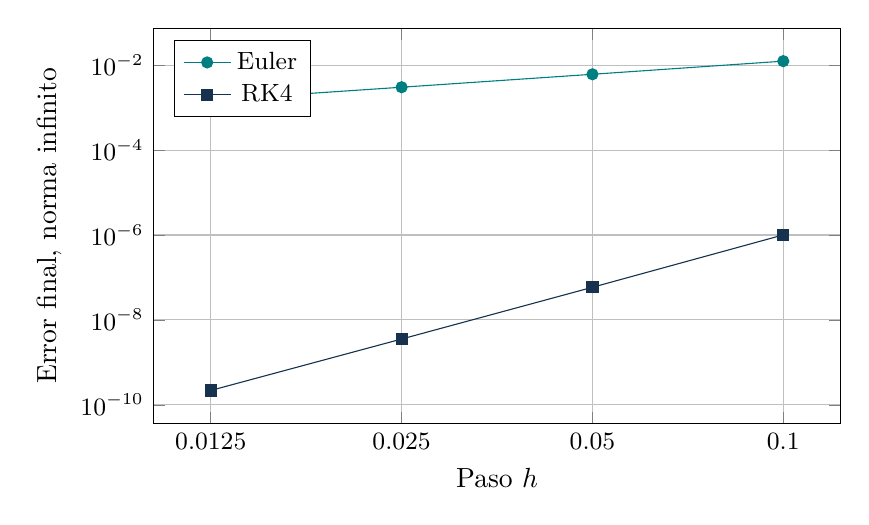
\begin{tikzpicture}
\begin{loglogaxis}[width=0.85\linewidth,height=6.6cm,xtick={0.0125,0.025,0.05,0.1},xticklabels={0.0125,0.025,0.05,0.1},minor x tick num=0,xlabel={Paso $h$},ylabel={Error final, norma infinito},grid=both,legend pos=north west,legend style={font=\small},tick label style={font=\small}]
\addplot[teal,mark=*] coordinates{(0.1,0.012489689888)(0.05,0.006131358824)(0.025,0.003037513478)(0.0125,0.00151174157)};
\addlegendentry{Euler}
\addplot[navy,mark=square*] coordinates{(0.1,1.006817743e-6)(0.05,5.876885986e-8)(0.025,3.549840588e-9)(0.0125,2.181144154e-10)};
\addlegendentry{RK4}
\end{loglogaxis}\end{tikzpicture}
\end{center}
Los órdenes se aproximan a uno y cuatro. Una comparación de costo usaría
cuatro veces más evaluaciones para RK4 a igual $h$; aun así, el error
obtenido en este ensayo es varios órdenes de magnitud menor.

\clearpage
\subsection{Adaptatividad con solución exacta para cualquier dato inicial}
Como verificación independiente se usa la familia
\[
u'=A(u-g(t))+g'(t),\qquad
u(t;z)=g(t)+e^{At}(z-g(0)),
\]
válida para cualquier $z\in\R^d$. Se toma
$g(t)=a\odot\sin(\nu t)+v\exp(-((t-1)/0.12)^2)$,
$a_i\in[0.2,0.6]$ y $v=\mathbf1/\sqrt d$.
El pulso suave exige mayor resolución cerca de $t=1$.
Se impone $h_{\max}=0.1$, $\atol=10^{-3}\rtol$ y se mide el máximo error
en todos los nodos aceptados. La exactitud de esta solución permite
verificar el código sin usar otro integrador como referencia.
\begin{center}\small
\begin{tabular}{@{}rrrrrr@{}}\toprule
$\rtol$ & Aceptados & Rechazos & Eval. $f$ & Error máx. & Máx. $r$\\\midrule
$10^{-3}$ & 20 & 0 & 240 & $4.727\cdot10^{-5}$ & 0.237\\
$10^{-5}$ & 28 & 6 & 408 & $3.631\cdot10^{-6}$ & 0.948\\
$10^{-7}$ & 56 & 15 & 852 & $1.121\cdot10^{-7}$ & 0.867\\
$10^{-9}$ & 138 & 22 & 1920 & $2.787\cdot10^{-9}$ & 0.987\\\bottomrule
\end{tabular}\end{center}
El error global disminuye al exigir menor tolerancia, pero no coincide
numéricamente con ella. A tolerancia $10^{-9}$, el máximo error absoluto es
$2.787\times10^{-9}$: el control local escalado no prometía una cota global
absoluta de $10^{-9}$. Los rechazos aumentan el costo y forman parte de la
medición, no deben omitirse al comparar métodos.

\subsection{Condiciones iniciales aleatorias y separación de errores}
Para comprobar transporte de momentos se toma $u'=Au$, $T=2$ y
$U_0\sim\mathcal N(\mu,\Sigma_0)$, con $\mu_i$ equiespaciados en
$[-0.4,0.5]$ y $\Sigma_0=0.04CC^\top$, donde $C$ es una matriz gaussiana
escalada por $1/\sqrt d$. Entonces
\[
m(T)=e^{AT}\mu,\qquad\Sigma(T)=e^{AT}\Sigma_0e^{A^\top T}.
\]
Se integran $M=20\,000$ realizaciones con RK4 fijo de $h=0.05$ y se
comparan con las soluciones exactas de \emph{las mismas} realizaciones.
El emparejamiento permite aislar error numérico de error de muestreo.
\begin{center}\small
\begin{tabularx}{\linewidth}{@{}Xr@{}}\toprule
Medición & Valor\\\midrule
RMS emparejado del error de trayectoria, norma euclídea & $3.292\cdot10^{-8}$\\
Error numérico de la media, norma euclídea & $2.699\cdot10^{-8}$\\
Error de muestreo de la media exacta & $7.284\cdot10^{-4}$\\
Error total de la media numérica & $7.284\cdot10^{-4}$\\
Error de muestreo de la covarianza, norma Frobenius & $1.719\cdot10^{-4}$\\
Error numérico de la covarianza emparejada & $2.412\cdot10^{-9}$\\\bottomrule
\end{tabularx}\end{center}
En este ensayo el error estadístico domina ampliamente. La coincidencia
redondeada del error total y del error de muestreo no implica identidad
exacta. El ejemplo gaussiano lineal se usa por disponer de momentos
exactos; la formulación y los algoritmos no presuponen esta distribución.

\textbf{Verificación conjunta de ambas extensiones.} En la auditoría se
integraron además 32 datos iniciales gaussianos con RK4 adaptativo sobre un
sistema no lineal acoplado de ocho variables, usando mallas independientes
y llegada exacta a $T=2$. Con $\rtol=10^{-7}$ y $\atol=10^{-10}$, el máximo
error final frente a DOP853 fue $7.638\times10^{-8}$. Las trayectorias
aceptaron entre 19 y 34 pasos, con 91 rechazos en total. Esta prueba confirma
el funcionamiento conjunto en la familia ensayada; la garantía general
sigue dependiendo de las hipótesis del teorema \ref{thm:lp}.

\clearpage
\subsection{Euler--Maruyama: acoplamiento y órdenes}
Como control de la distinción estocástica, se simula
$\mathrm dX=-0.3X\,\mathrm dt+0.7X\,\mathrm dW$, $X(0)=1$, $T=1$.
Su solución exacta es $X(1)=\exp((-0.3-0.7^2/2)+0.7W(1))$.
Con $M=12\,000$ caminos se generan incrementos en la malla fina de
$1024$ pasos. Los incrementos gruesos se obtienen sumando bloques de los
incrementos finos, de modo que todos los métodos comparten cada realización
browniana. Se mide $[M^{-1}\sum_j|X_N^{(j)}-X^{(j)}(1)|^2]^{1/2}$.
\begin{center}\small
\begin{tabular}{@{}rrrr@{}}\toprule
Pasos & RMSE fuerte & Orden observado & Sesgo débil exacto de la media\\\midrule
32 & $5.8791\cdot10^{-2}$ & --- & $1.0476\cdot10^{-3}$\\
64 & $4.0221\cdot10^{-2}$ & 0.548 & $5.2234\cdot10^{-4}$\\
128 & $2.8799\cdot10^{-2}$ & 0.482 & $2.6081\cdot10^{-4}$\\
256 & $2.0681\cdot10^{-2}$ & 0.478 & $1.3031\cdot10^{-4}$\\
512 & $1.4666\cdot10^{-2}$ & 0.496 & $6.5134\cdot10^{-5}$\\
1024 & $1.0273\cdot10^{-2}$ & 0.514 & $3.2561\cdot10^{-5}$\\\bottomrule
\end{tabular}\end{center}
El sesgo débil de esta tabla se calcula analíticamente como
$|(1-0.3h)^{1/h}-e^{-0.3}|$. Así se evita confundirlo con la fluctuación
de una media Monte Carlo. El orden fuerte se aproxima a $1/2$, mientras
el sesgo débil se reduce por un factor cercano a dos al dividir $h$ por dos.
Este test escalar verifica el tratamiento del ruido; la función
Euler--Maruyama entregada admite $d$ y $m$ arbitrarios.

\subsection{Límites de la evidencia computacional}
Los resultados son cálculos ejecutados, no cifras copiadas de los artículos.
Muestran consistencia con las tasas teóricas en familias suaves y con
referencias controladas. No prueban convergencia para todo sistema ni
evalúan universalmente el estado del arte. Quedan fuera eventos,
discontinuidades, problemas de alta rigidez, ruido no browniano y leyes de
colas pesadas sin suficientes momentos. La prueba general depende de las
hipótesis establecidas, no de extrapolar estas tablas a esos regímenes.

\section{Conclusiones y líneas de trabajo}
RK4 conserva su construcción y su orden en dimensión arbitraria cuando
el campo satisface las condiciones de regularidad y estabilidad apropiadas.
Con dato inicial aleatorio, el algoritmo transporta realizaciones de una
misma ley inicial; las garantías $L^p$ requieren integrabilidad de las
constantes de error. La duplicación de paso proporciona un estimador
transparente con factor $15$, pero su costo y su carácter local motivan
comparación con pares embebidos y estimadores globales por residuos.

La revisión muestra conexiones útiles con filtros probabilísticos,
controladores PI/PID y preservación geométrica. Cada línea resuelve un
problema específico y debe evaluarse bajo sus propias hipótesis. Para
continuar, conviene comparar error frente a evaluaciones del campo con
Dormand--Prince, estudiar sensibilidad a la ley de $U_0$ y probar
controladores PI frente a I sobre familias rígidas y no rígidas. Una futura
extensión estocástica adaptativa debe preservar los incrementos brownianos
al refinar, en vez de reutilizar sin justificación el rechazo determinista.

\clearpage
\renewcommand{\refname}{Referencias verificables}
\phantomsection
\addcontentsline{toc}{section}{Referencias verificables}
\small
\begin{thebibliography}{99}
\bibitem{hairer} E. Hairer, S. P. Nørsett y G. Wanner (1993).
\emph{Solving Ordinary Differential Equations I: Nonstiff Problems}, 2.ª ed.
Springer. \url{https://doi.org/10.1007/978-3-540-78862-1}.
\bibitem{dormand} J. R. Dormand y P. J. Prince (1980).
\emph{A family of embedded Runge--Kutta formulae}.
Journal of Computational and Applied Mathematics 6(1), 19--26.
\url{https://doi.org/10.1016/0771-050X(80)90013-3}.
\bibitem{higham} D. J. Higham (2001).
\emph{An Algorithmic Introduction to Numerical Simulation of Stochastic Differential Equations}.
SIAM Review 43(3), 525--546.
\url{https://doi.org/10.1137/S0036144500378302}.
\bibitem{schober} M. Schober, D. Duvenaud y P. Hennig (2014).
\emph{Probabilistic ODE Solvers with Runge--Kutta Means}.
NeurIPS 2014. \url{https://arxiv.org/abs/1406.2582} (v2).
\bibitem{conrad} P. R. Conrad, M. Girolami, S. Särkkä, A. Stuart y K. Zygalakis (2015).
\emph{Probability Measures for Numerical Solutions of Differential Equations}.
Preprint. \url{https://arxiv.org/abs/1506.04592}.
Versión de revista relacionada: \emph{Statistical analysis of differential equations:
introducing probability measures on numerical solutions}, Statistics and Computing
27, 1065--1082 (2017).
\bibitem{kruse} R. Kruse y Y. Wu (2017).
\emph{Error analysis of randomized Runge--Kutta methods for differential equations with time-irregular coefficients}.
Computational Methods in Applied Mathematics 17(3), 479--498.
\url{https://arxiv.org/abs/1701.03444} (v2).
\bibitem{abdulle} A. Abdulle y G. Garegnani (2020).
\emph{Random time step probabilistic methods for uncertainty quantification in chaotic and geometric numerical integration}.
Statistics and Computing 30, 907--932.
\url{https://arxiv.org/abs/1801.01340} (v4).
\bibitem{bosch} N. Bosch, P. Hennig y F. Tronarp (2021).
\emph{Calibrated Adaptive Probabilistic ODE Solvers}.
AISTATS, Proceedings of Machine Learning Research 130, 3466--3474.
\url{https://arxiv.org/abs/2012.08202} (v2).
\bibitem{ranocha2024} H. Ranocha y J. Giesselmann (2024).
\emph{Stability of step size control based on a posteriori error estimates}.
Computational Science and Engineering.
\url{https://arxiv.org/abs/2307.12677} (v3).
\url{https://doi.org/10.1007/s44207-024-00001-0}.
\bibitem{bleecke} S. Bleecke y H. Ranocha (2023).
\emph{Step size control for explicit relaxation Runge--Kutta methods preserving invariants}.
Preprint. \url{https://arxiv.org/abs/2311.14050}.
\bibitem{wu} M. Wu y M. Lysy (2025).
\emph{rodeo: Probabilistic Methods of Parameter Inference for Ordinary Differential Equations}.
Preprint. \url{https://arxiv.org/abs/2506.21776} (v1).
\bibitem{connected} Connected Papers. Grafo público localizado de
\emph{Probabilistic linear solvers: a unifying view}.
Consulta: 13 de octubre de 2026. Usado como pista bibliográfica, no como
fuente de resultados matemáticos ni exportación de grafo.
\href{https://www.connectedpapers.com/main/ee71541a36a170d0fafb881faf661e00f4df9a48/Probabilistic-linear-solvers:-a-unifying-view/graph}{Enlace al grafo público}.
\end{thebibliography}
\end{document}
